\section{Practical cases}

\begin{frame}{}
    \tableofcontents[currentsection]
\end{frame}

% ------------------------------------------
\subsection{Fundamental 6-bus case}
% \begin{frame}{}
%     \tableofcontents[currentsection]
% \end{frame}


\begin{frame}{GUI usage: modelling}
    \fbox{python -c "from GridCal.ExecuteGridCal import runGridCal; runGridCal()"}

    \begin{columns}
        \begin{column}{0.65\textwidth}
    \begin{figure}[H]
        \centering
    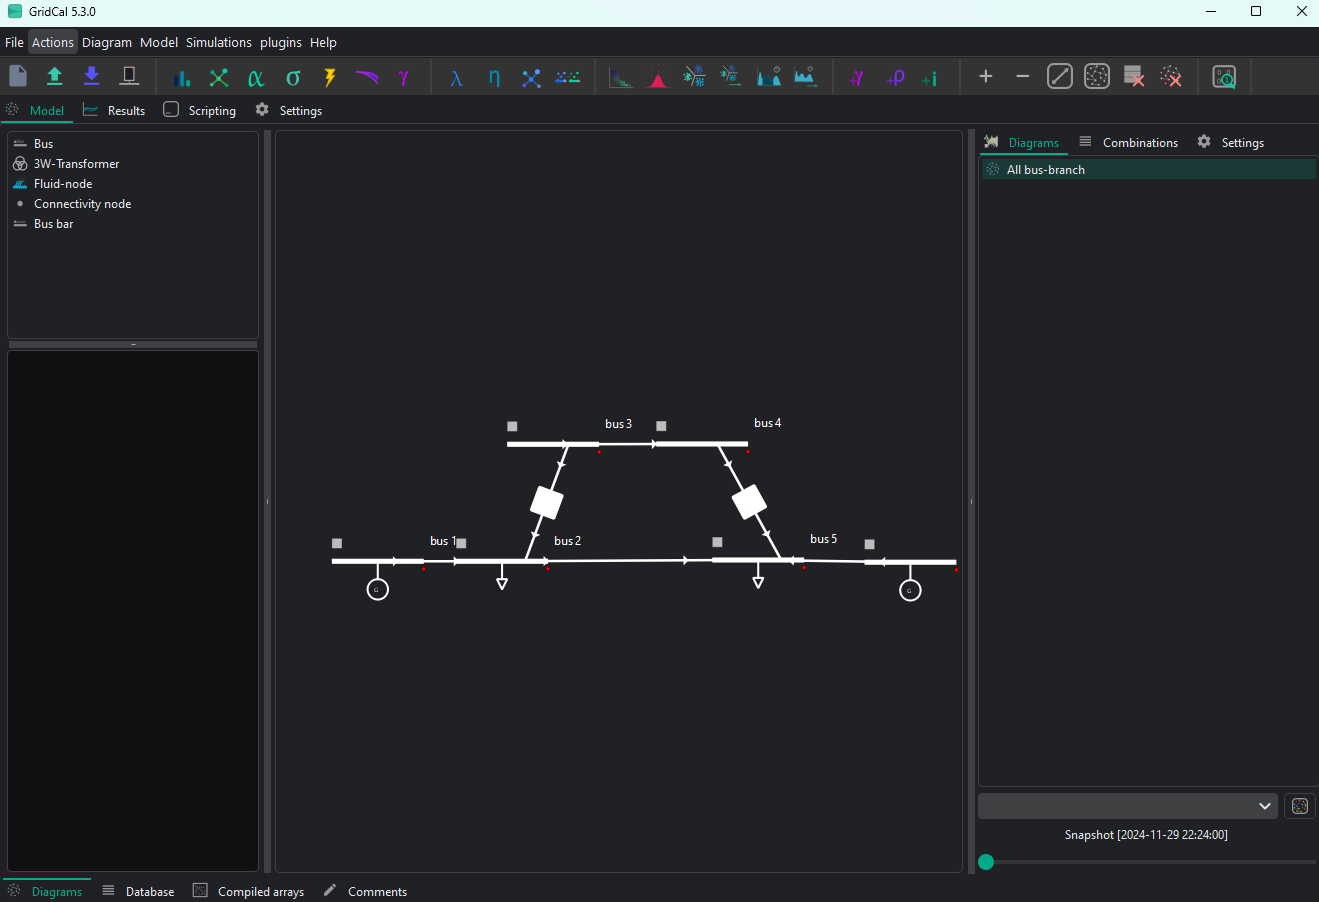
\includegraphics[width=0.99\textwidth]{Images/6busgui.png}
    \caption{Visualization of the 6-bus grid through the GUI.}
    \label{fig:6bus1}
    \end{figure}
        \end{column}
        
        \begin{column}{0.35\textwidth}
            \begin{itemize}
                \item Go over the complete database.
                \item Check the controls of the generators.
                \item Check the controls of the VSCs. What to expect?
            \end{itemize}
        \end{column}
    \end{columns}
\end{frame}

\begin{frame}{GUI usage: solving}
    % solver selection screen and results table
    \begin{figure}[H]
        \centering
    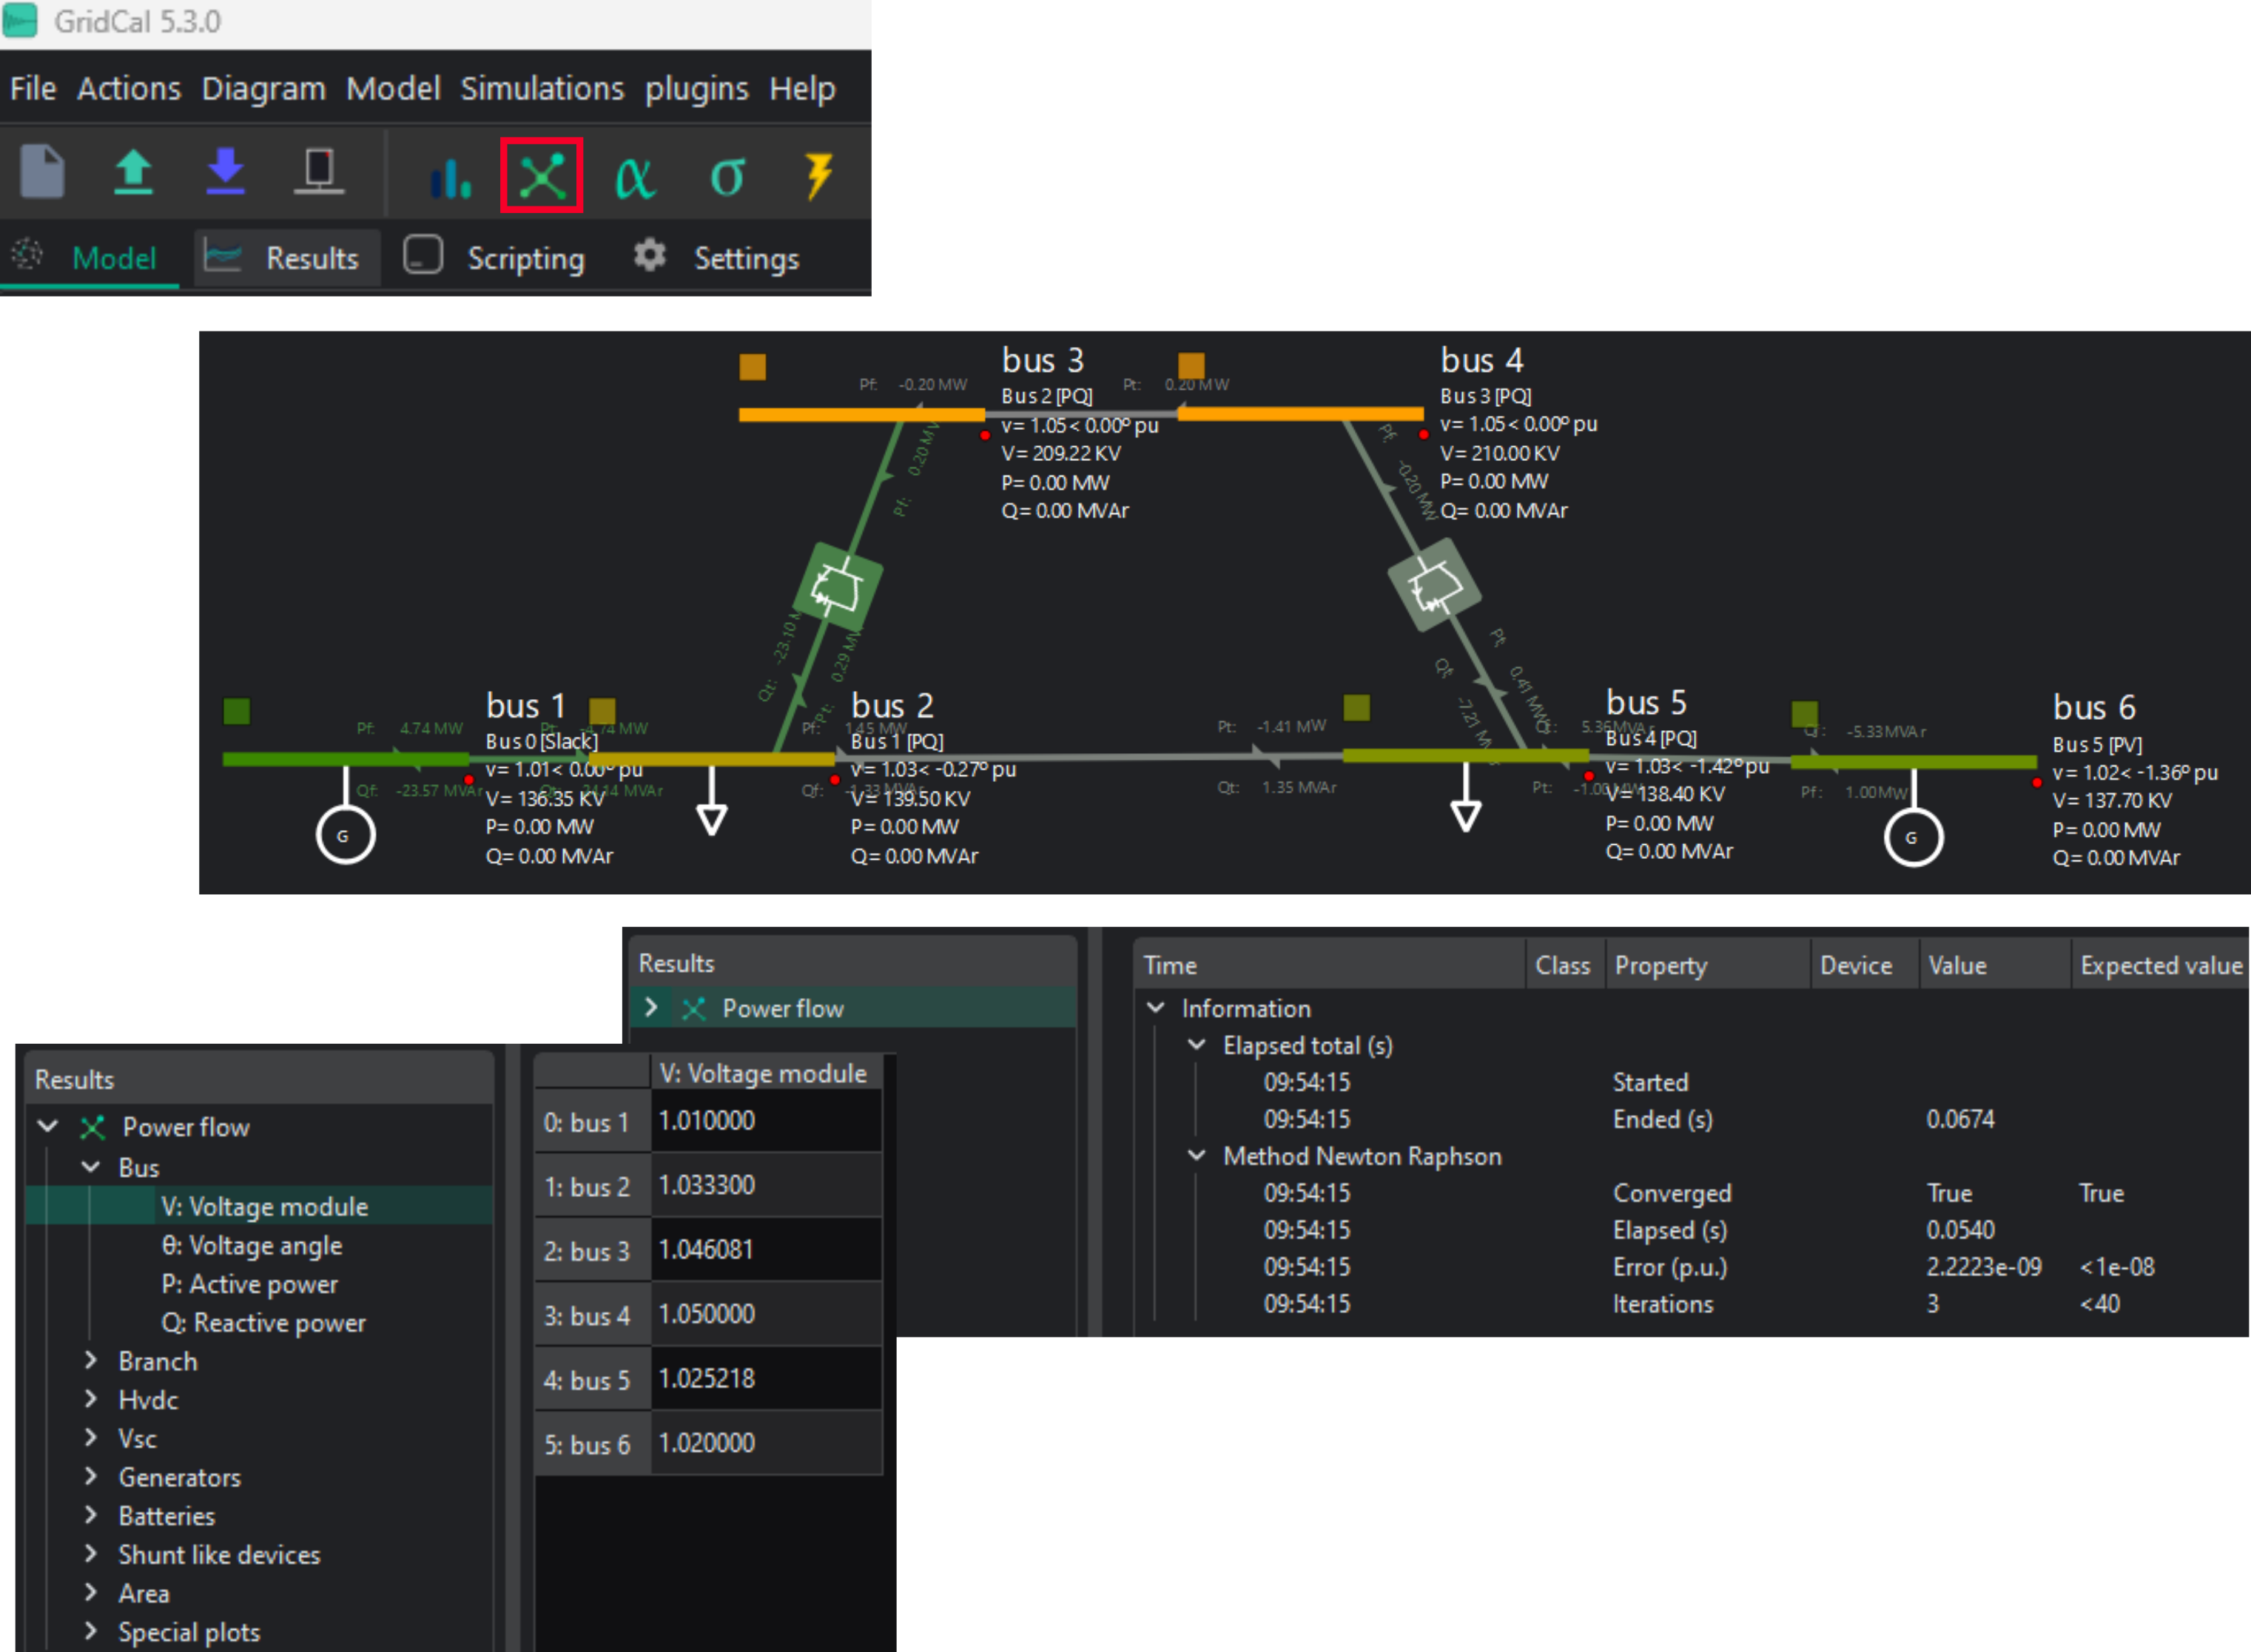
\includegraphics[width=0.75\textwidth]{Images/6busgui2.png}
    \caption{GUI simulation execution, solver selection and results visualization on the 6-bus grid.}
    \label{fig:6bus2}
    \end{figure}
\end{frame}

\begin{frame}{A few questions}
    Solver selection:
    \begin{itemize}
        \item Run the power flow with both the Newton-Raphson and the Gauss-Seidel.
        \item How many iterations do we need in both?
        \item What is the computational time?
    \end{itemize}
    Control setting:
    \begin{itemize}
        \item What if the two converters control active power?
        \item What if the two converters control voltage on the DC side?
    \end{itemize}
\end{frame}

\begin{frame}[fragile]{Scripting: modelling}
   % nothing, just work on the jupyter notebook 
   \begin{itemize}
    \item Let's move into our code editor.
   \end{itemize}

    \begin{lstlisting}[language=Python]
import numpy as np
import GridCalEngine as gce
from GridCalEngine.enumerations import ConverterControlType

# Grid instantiation
grid = gce.MultiCircuit()

# Define buses
bus1 = gce.Bus(name='B1', Vnom=135, is_slack=True)
...
    \end{lstlisting}
\end{frame}

\begin{frame}[fragile]{Scripting: solving}
   % nothing, just work on the jupyter notebook 
    \begin{itemize}
    \item Let's move into our code editor.
    \end{itemize}
    \begin{lstlisting}[language=Python]
pf_driver = gce.PowerFlowDriver(grid=grid)
pf_driver.run()
Vm = pf_driver.results.voltage
Va = np.angle(pf_driver.results.voltage, deg=True)
    \end{lstlisting}
\end{frame}

% ------------------------------------------
\subsection{Interconnected 17-bus case}
% \begin{frame}{}
%     \tableofcontents[currentsection]
% \end{frame}

\begin{frame}{Challenges of advanced cases}
    \begin{columns}
        
        \begin{column}{0.49\textwidth}
            \begin{itemize}
                \item The 6-bus case had 1 AC and 1 DC subsystem.
                \item Transnational grids are composed of many AC and DC grids.
                \item Real grids may also have controllable transformers.
            \end{itemize}
        \end{column}

        \begin{column}{0.5\textwidth}
            \begin{figure}[H]
                \centering
            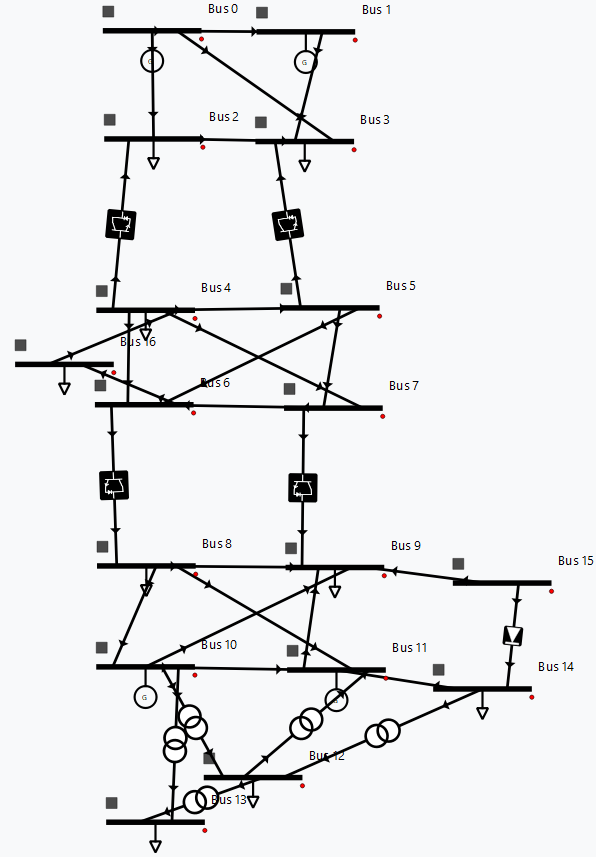
\includegraphics[width=0.73\textwidth]{Images/17busgui1.png}
            \caption{Interconnected AC systems overview.}
            \label{fig:17bus1}
            \end{figure}
        \end{column}

    \end{columns}

\end{frame}

\begin{frame}{Issues in the 17-bus cases}
    What issues are we facing?
    \begin{figure}[H]
        \centering
    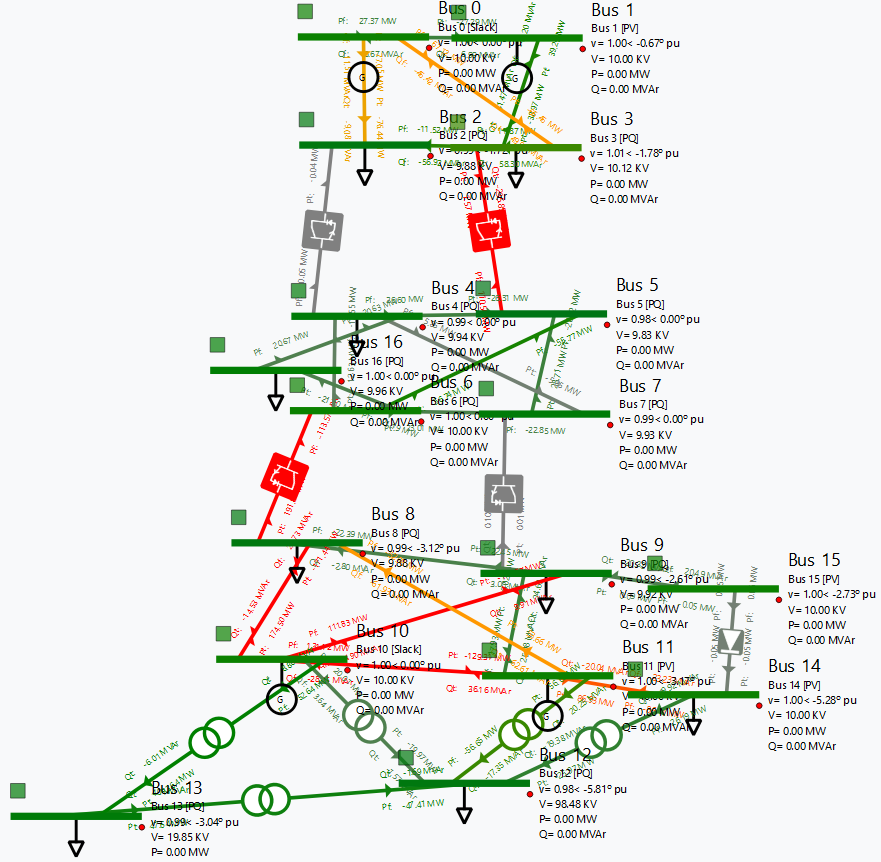
\includegraphics[width=0.52\textwidth]{Images/17bus_issues.png}
    \caption{Default interconnected AC system results.}
    \label{fig:17bus2}
    \end{figure}
\end{frame}

\begin{frame}{Fixing issues in the 17-bus cases}
    \begin{columns}
        
        \begin{column}{0.49\textwidth}
            Some potential fixes include:
            \begin{itemize}
                \item Adjust the transformer control setpoints.
                \item Change the VSCs control modes.
                \item Modify the VSCs control setpoints.
                \item Regulate the generators voltage reference.
            \end{itemize}
        \end{column}

        \begin{column}{0.5\textwidth}
            \begin{figure}[H]
                \centering
            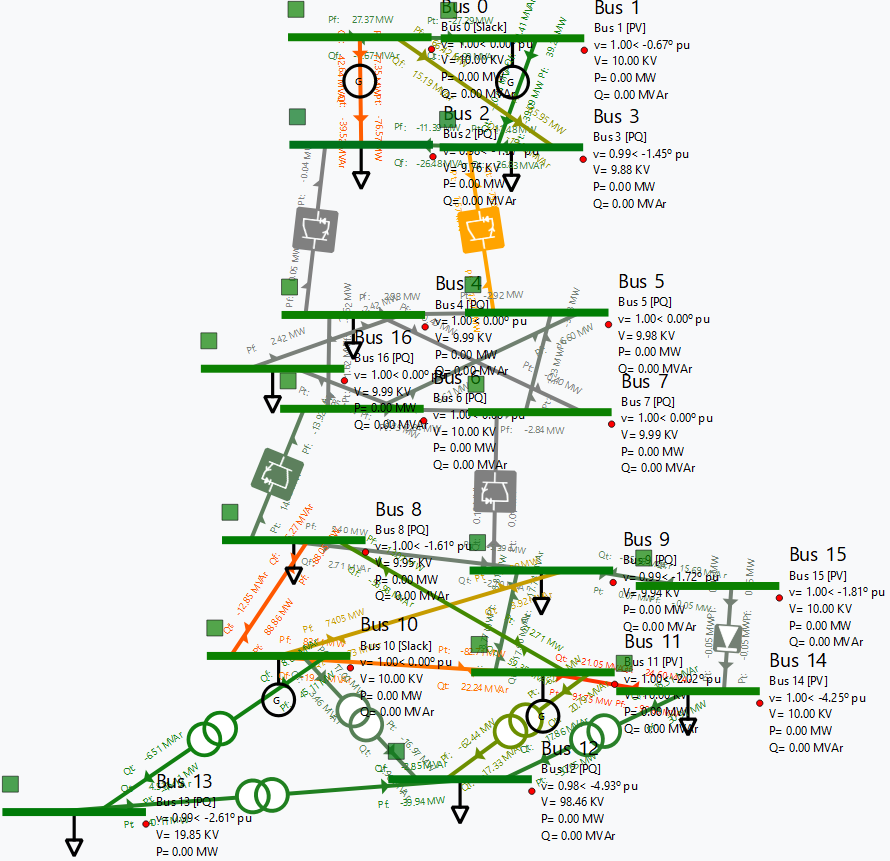
\includegraphics[width=0.93\textwidth]{Images/17bus_solved.png}
            \caption{Interconnected AC systems with a feasible solution.}
            \label{fig:17bus3}
            \end{figure}
        \end{column}
    \end{columns}
\end{frame}

\begin{frame}{Transformer control}

    \begin{columns}
        
        \begin{column}{0.5\textwidth}
    Despite being less flexible than VSCs, some transformers are also controllable:
    \begin{itemize}
        \item $m$: the tap module can regulate $V_m$ and $Q$
        \item $\tau$: the tap angle can adjust $P$
    \end{itemize}
    \begin{figure}[!htb]
        \centering
        \begin{circuitikz}[american]
            \draw[line width=0.7mm] (2,-1) to [short] (2,-2);
            \draw[line width=0.7mm] (7,-1) to [short] (7,-2);
            % \draw (2,-1.5) to [cute inductor, l=$m\angle \tau$] (7,-1.5);
            % \draw (2,-1.5) circle (0.3cm);
            % \draw (4.5,-1.5) circle (0.3cm);
            \draw (4.75,-1.5) circle (0.3cm);
            \draw (4.25,-1.5) circle (0.3cm);
            \node at (4.5,-1.0) {$m\angle \tau$};
            \draw (2,-1.5) to [short, i_=$P_f+jQ_f$]  (3.95,-1.5);
            \draw (7,-1.5) to [short, i=$P_t+jQ_t$]  (5.05,-1.5);
            \node at (2,-0.65) {$V_f \angle \delta_f$};
            \node at (7,-0.65) {$V_t \angle \delta_t$};
        \end{circuitikz}
        \caption{Representation of a controllable transformer.}
    \end{figure}
        \end{column}

        \begin{column}{0.5\textwidth}
            \begin{itemize}
            \item Let's increase $V_{m,13}$ to $1.019876$~p.u..
            \item Is it reasonable to have $0.9 \leq m \leq 1.0$?
            \end{itemize}
            \begin{figure}[H]
                \centering
            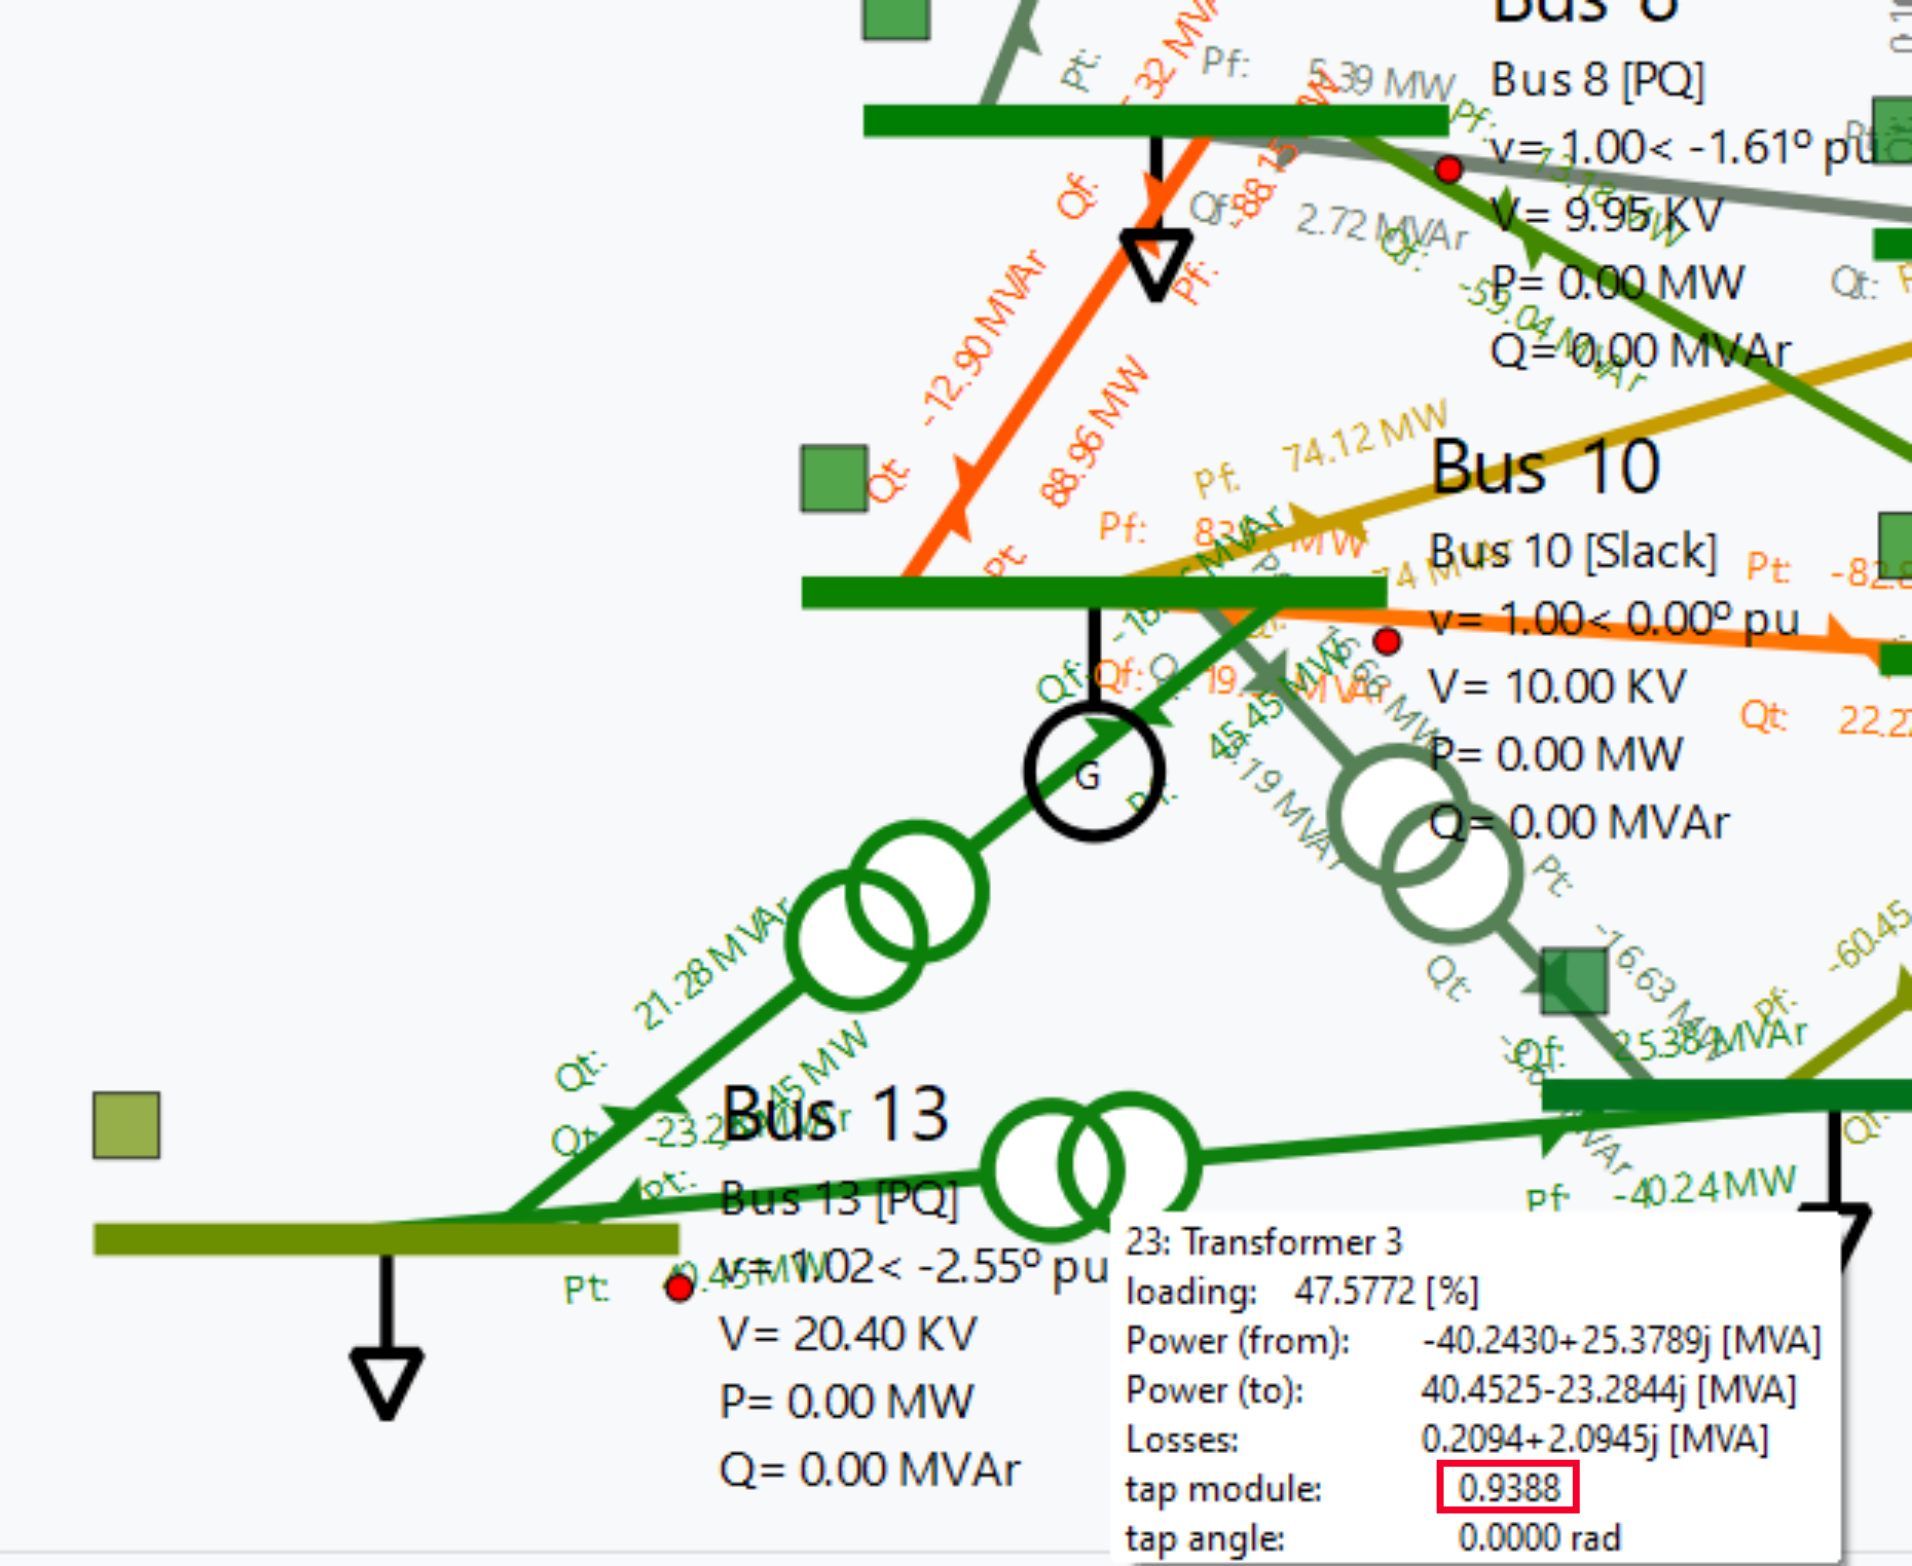
\includegraphics[width=0.85\textwidth]{Images/17bus_trafo.png}
            \caption{Transformer controlling $V_m$ with $m$.}
            \label{fig:17bus3}
            \end{figure}
        \end{column}
    \end{columns}
\end{frame}

% show how slow it goes with autodiff
% test setting some Va for grid-forming
% helm to get a feeling of solvability

% ------------------------------------------
\subsection{IEEE 118-bus case}
% first run HELM sigma and see we are getting some issues
% then add VSCs linking systems and show improvement in V profile

\begin{frame}{What is a large system?}
      \begin{figure}[H]
        \centering
    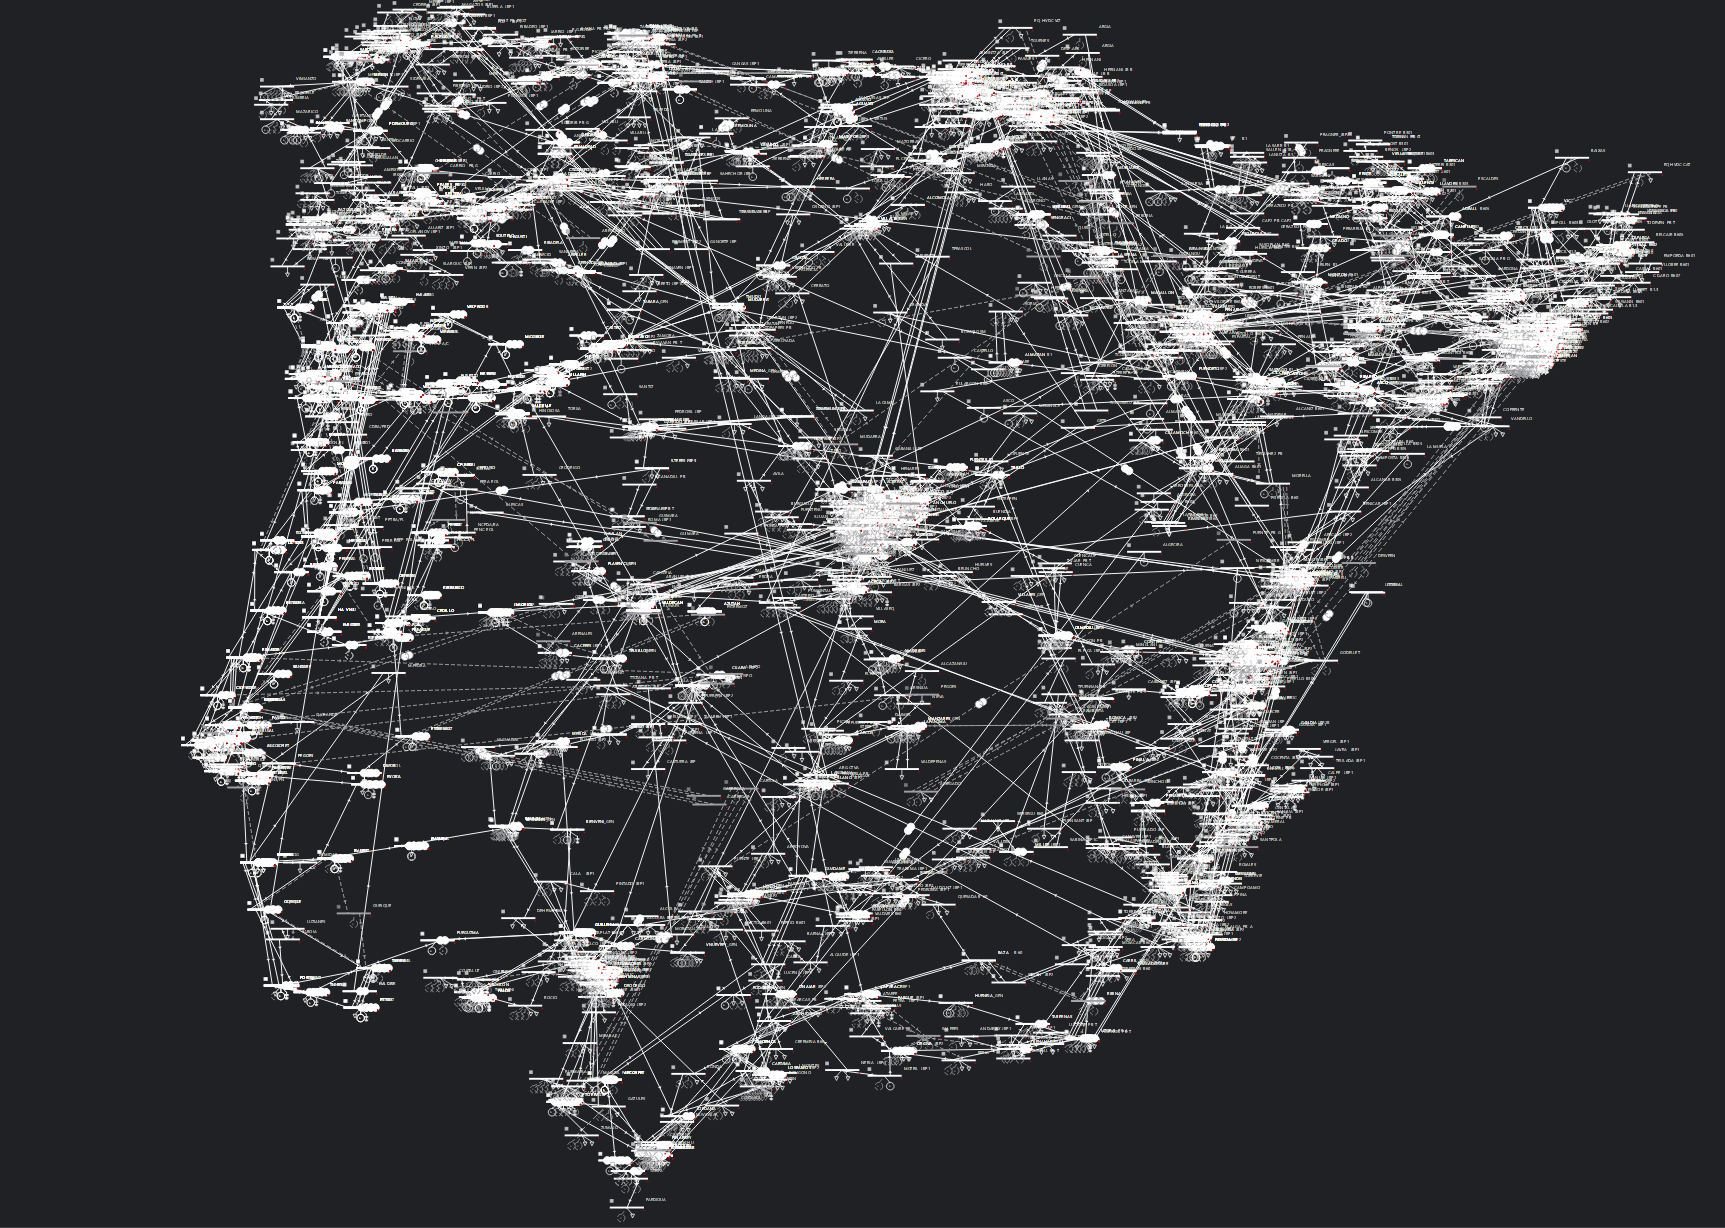
\includegraphics[width=0.75\textwidth]{Images/ESPgrid_topo.png}
    \caption{Grid topology of the Iberian system.}
    \label{fig:peninsula}
    \end{figure}   

\end{frame}

\begin{frame}{What is a large system?}
  \begin{itemize}
    \item Note: open the grid of Las Palmas to exemplify.
  \end{itemize} 
      \begin{figure}[H]
        \centering
    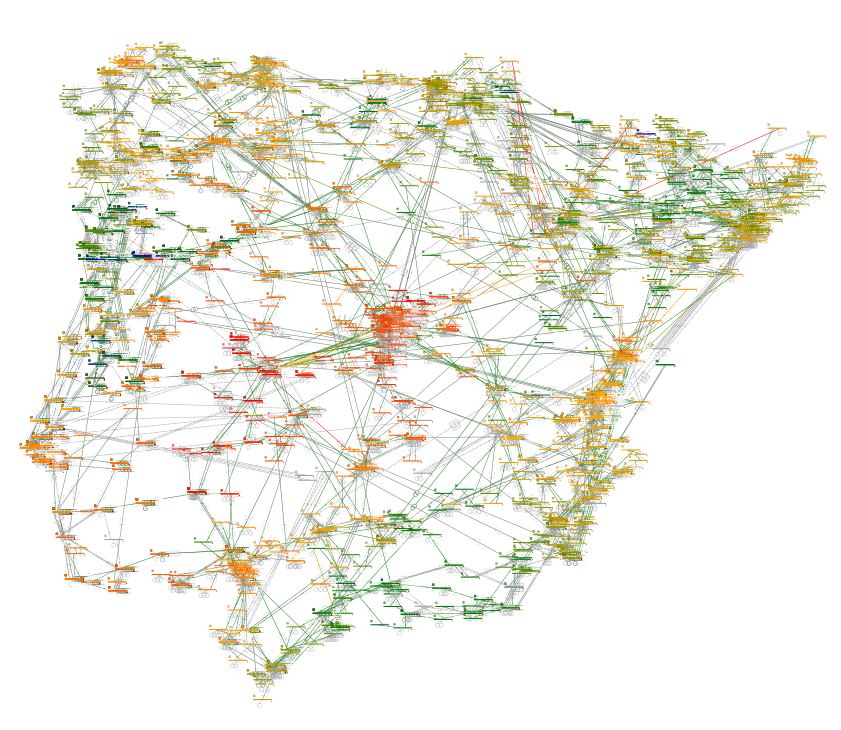
\includegraphics[width=0.60\textwidth]{Images/ESPgrid_solved.png}
    \caption{Solved power flow for the Iberian system.}
    \label{fig:peninsula2}
    \end{figure}   
\end{frame}

\begin{frame}{IEEE 118-bus operational overview}
    \begin{columns}
        
        \begin{column}{0.4\textwidth}
            \begin{itemize}
                \item Are voltage magnitudes correct?
                \item Are branch loadings within limits?
                \item How could an AC/DC link help?
            \end{itemize}
        \end{column}

        \begin{column}{0.45\textwidth}
     \begin{figure}[H]
        \centering
    % 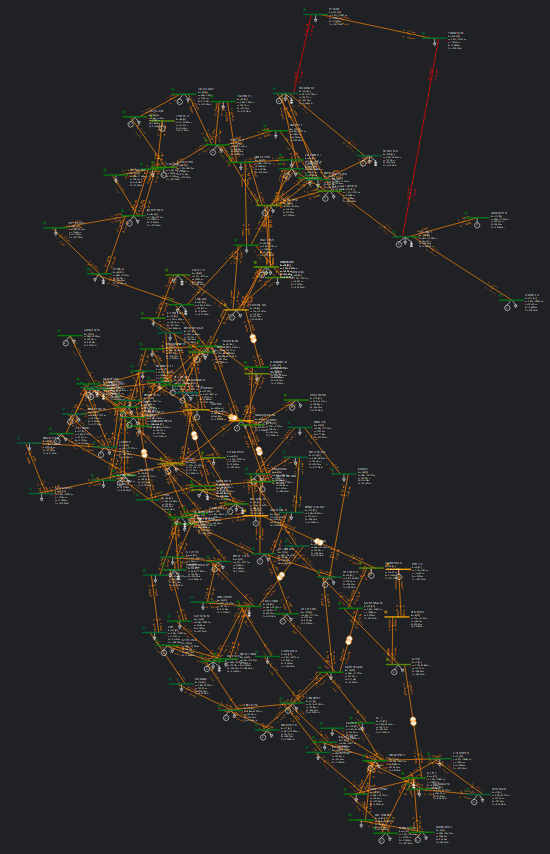
\includegraphics[width=0.65\textwidth]{Images/ie118_overscheme.png}
    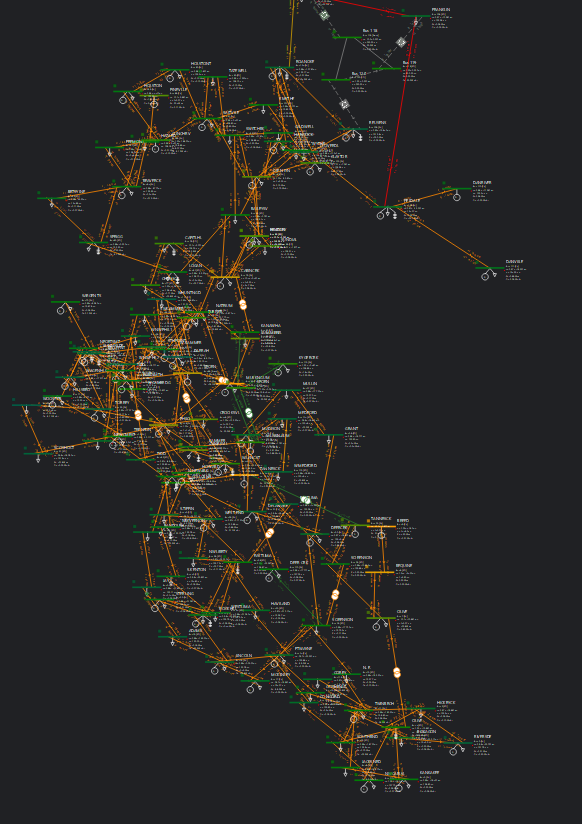
\includegraphics[width=0.80\textwidth]{Images/ie18_oper_v3.png}
    \caption{Original operation of the IEEE 118-bus grid.}
    \label{fig:118op}
    \end{figure}   
        \end{column}
    \end{columns}

\end{frame}

\begin{frame}{HELM analysis}
    \begin{figure}[H]
        \centering
    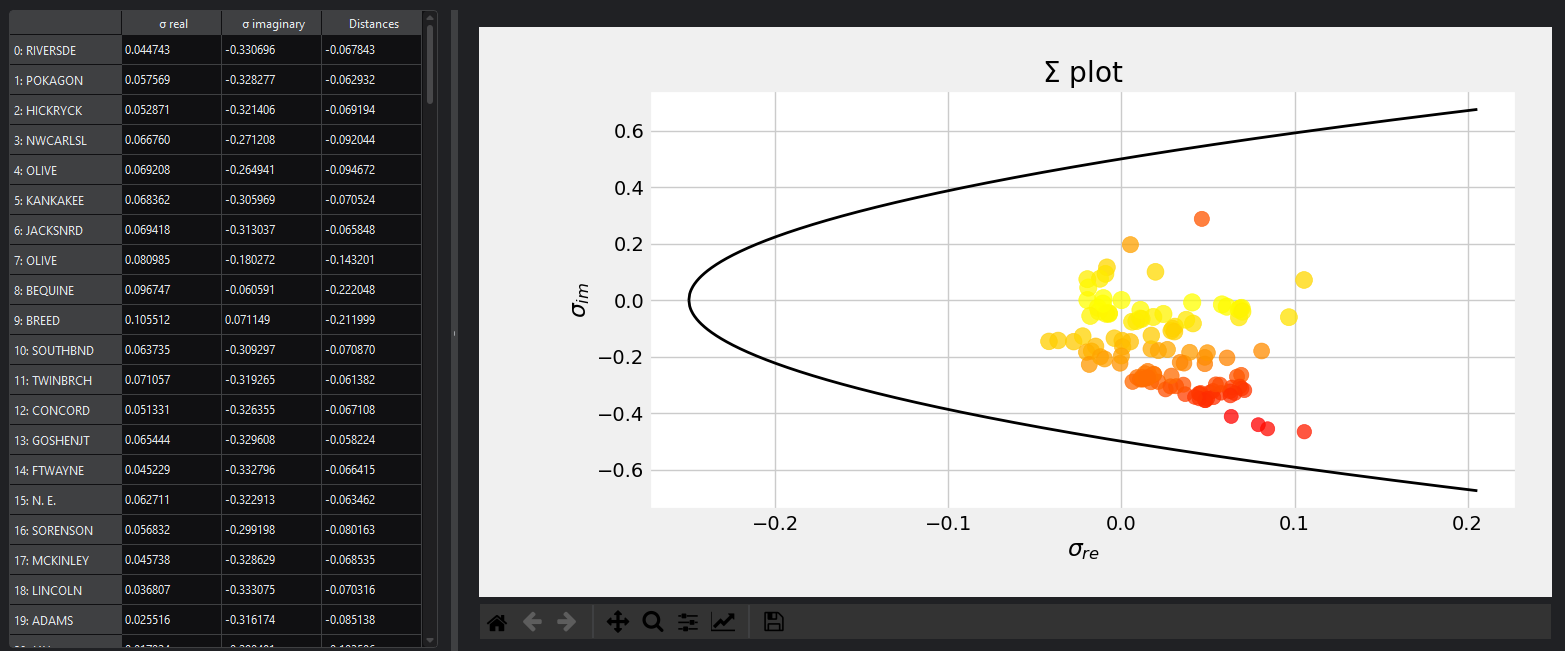
\includegraphics[width=0.99\textwidth]{Images/sigma_ie1182.png}
    \caption{HELM's Sigma plot showing showing the complicated feasibility of the systems.}
    \label{fig:118helm}
    \end{figure}
\end{frame}

\begin{frame}{Voltage and branch loading profiles}
    \begin{figure}[H]
        \centering
    % 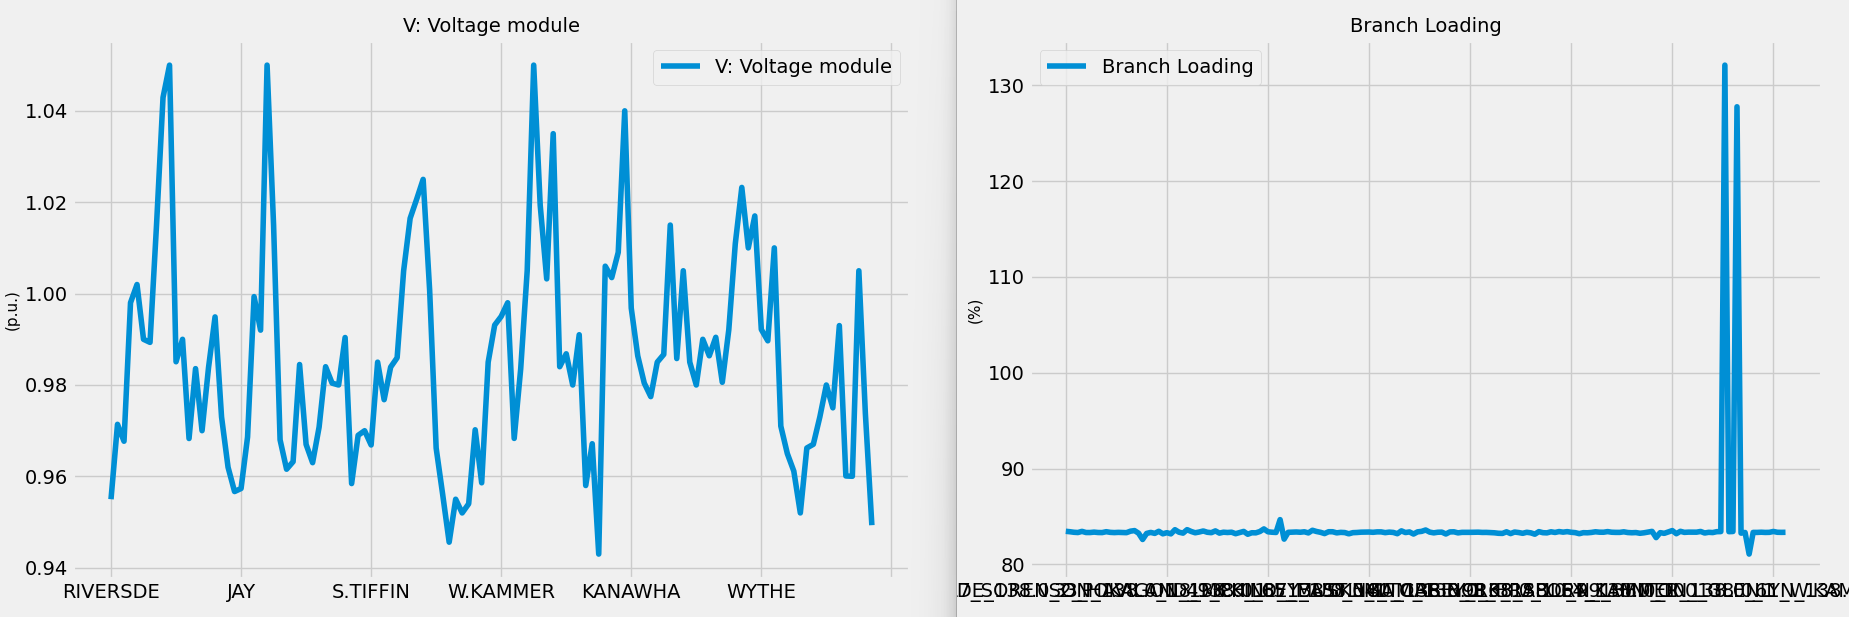
\includegraphics[width=0.99\textwidth]{Images/ie118_over.png}
    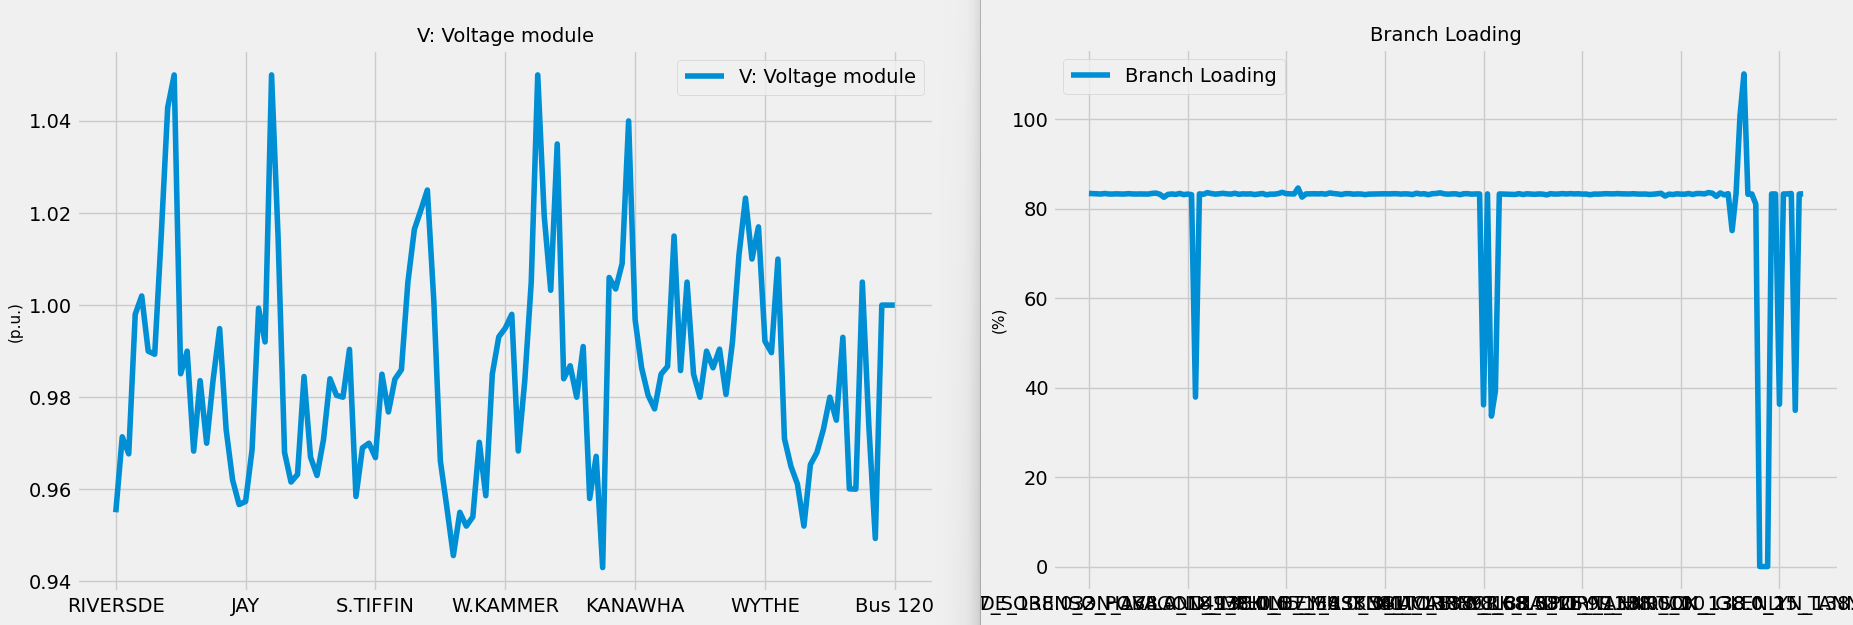
\includegraphics[width=0.99\textwidth]{Images/vl_ie18_v3.png}
    \caption{Voltage and branch loadings for the whole IEEE 118-bus system.}
    \label{fig:118vl}
    \end{figure}
\end{frame}

\begin{frame}{VSCs control management}
    \begin{figure}[H]
        \centering
    % 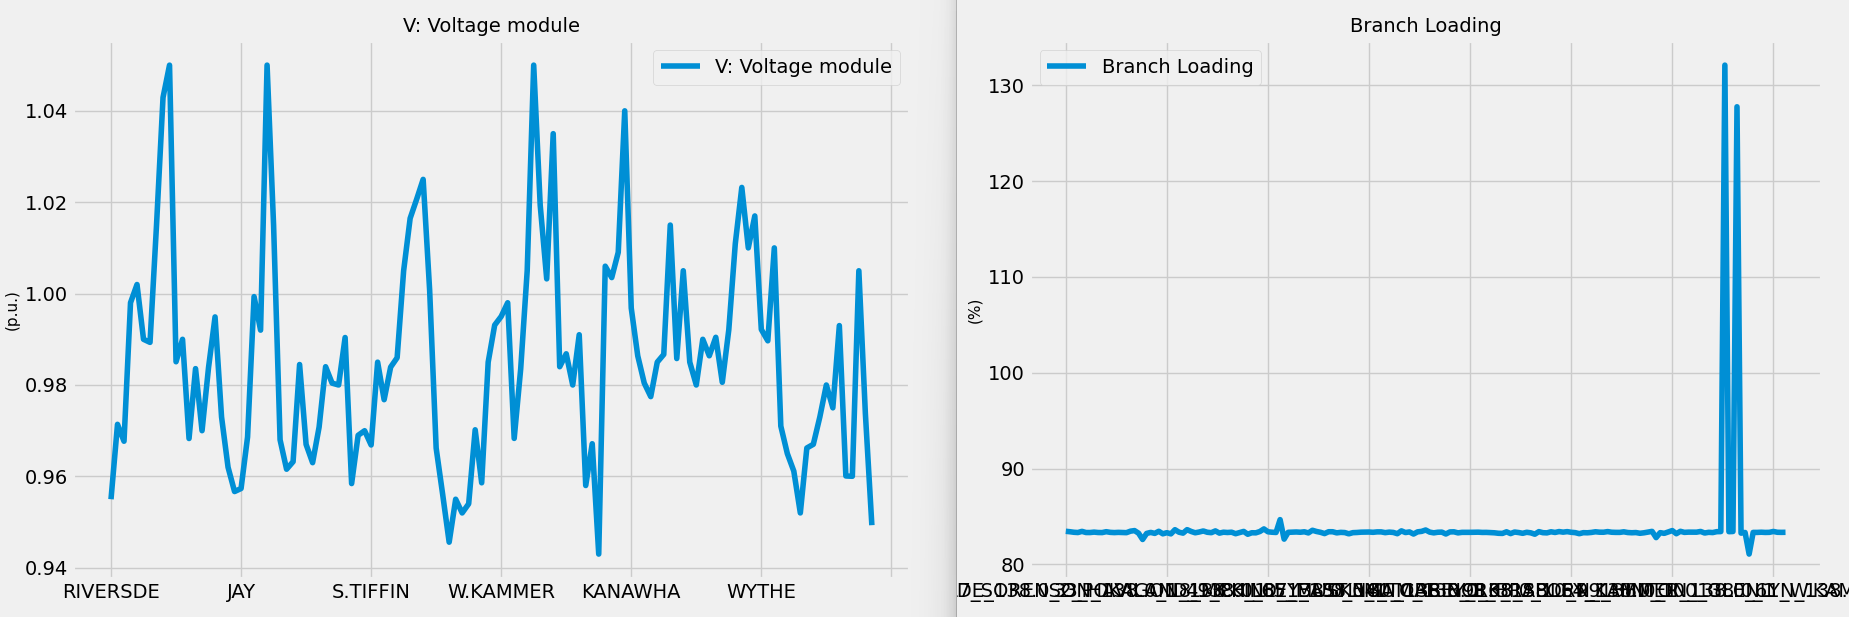
\includegraphics[width=0.99\textwidth]{Images/ie118_over.png}
    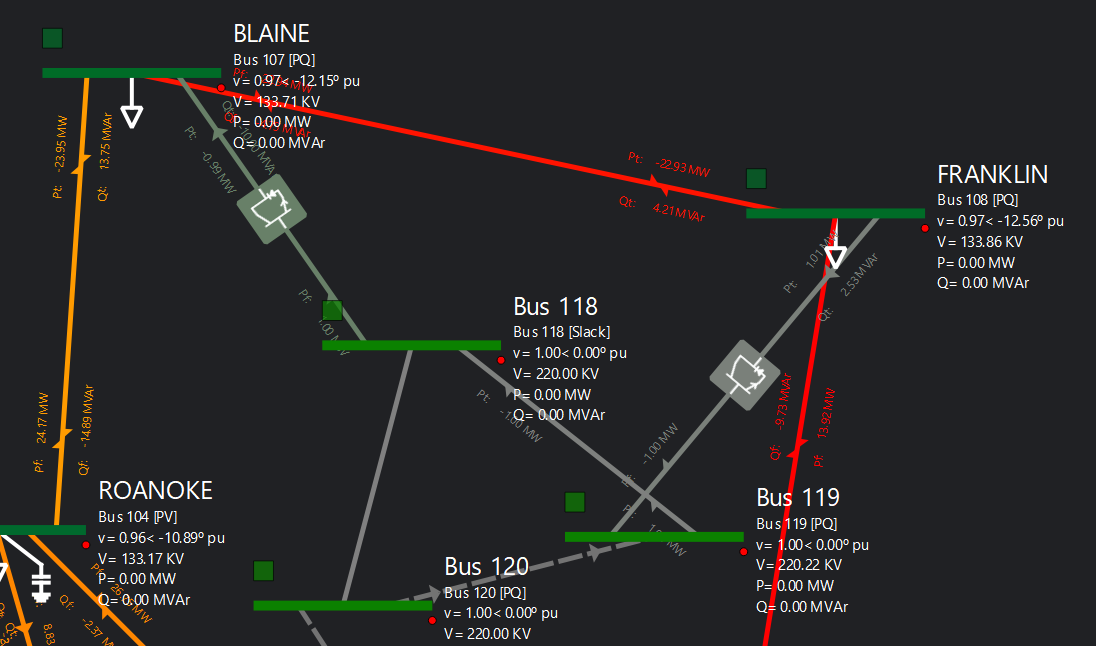
\includegraphics[width=0.90\textwidth]{Images/ie18_v3_fixed.png}
    \caption{Potential AC/DC link configuration.}
    \label{fig:118acdc}
    \end{figure}
\end{frame}






% \begin{frame}{}
%     \tableofcontents[currentsection]
% \end{frame}

% add some AC/DC vscs, show we solve it fast
% try the same with Gauss-Seidel and others. The way it is build should be straightfoward!?
